\documentclass{tufte-handout}
\usepackage{graphicx}
\usepackage{exercise}
\usepackage{enumerate}
\usepackage{mathtools}
\usepackage{amsmath,amssymb,amsthm}
\usepackage{enumitem}
%\usepackage{subcaption}
\usepackage{caption}
\usepackage{float}
\usepackage{hyperref}
\hypersetup{
    colorlinks = true,
    linkbordercolor = {white},
}
\usepackage{tikz}
\usepackage[numbered, framed]{matlab-prettifier}

% Silence warnings from tufte-handout bibliography handling
\usepackage{silence}
\WarningFilter{latex}{File `dummy.bib'}
\begin{filecontents*}{dummy.bib}
\end{filecontents*}
\WarningsOff[natbib]
\WarningsOff[bibentry]
\bibliographystyle{plainnat}

\newcommand{\bi}{\begin{itemize}}
\newcommand{\ei}{\end{itemize}}
\newcommand{\be}{\begin{enumerate}}
\newcommand{\ee}{\end{enumerate}}
\newcommand{\beq}{\begin{equation}}
\newcommand{\eeq}{\end{equation}}
\newcommand{\foo}[1]{%
\begin{tikzpicture}[#1]%
    \includegraphics[width=0.3cm]{figs/MatlabLogo.png}
\end{tikzpicture}%
}
\newcommand{\fuh}[1]{%
\begin{tikzpicture}[#1]%  x
    \includegraphics[width=0.3cm]{figs/MathematicaLogo.png}
\end{tikzpicture}%
}
\newcommand{\fie}[1]{%
\begin{tikzpicture}[#1]%
    \includegraphics[width=0.3cm]{figs/SolidworksLogo.png}
\end{tikzpicture}%
}
\let\ph\mlplaceholder % shorter macro
\lstMakeShortInline"

\lstset{
  style              = Matlab-editor,
  basicstyle         = \mlttfamily,
  escapechar         = ",
  mlshowsectionrules = true,
}


\title{Eigen Math \& Frequency Analysis for Audio}
\author{}
\date{\today}

\begin{document}

\maketitle

\vspace{0.1in}

% ----- Learning Goals -----
\section{Learning Goals}

\begin{description}[font=$\bullet$\scshape\bfseries]

\item[]Review Principal Component Analysis

\item[]Understand the difference between correlation and covariance matrices and how they are applied in different situations. 

\item[]Understand what Singular Value Decomposition(SVD) yields and learn how to implement it in MATLAB.

\item[]Review DFT and explore its possible applications such as noise removal and spectral subtraction filtering.

\item[]Review basic signal processing concepts such as the Nyquist Theorem.

\item[]Apply the knowledge from facial recognition and implement for voice classification using MATLAB.

\end{description}


% ----- Eigen-Math Review -----

\section{Eigen Analysis Revisited (3 hours)}

\subsection{What did we learn?}
During QEA I Module II, we learned how to recognize faces by conducting Principal Component Analysis, also known as Eigenfaces method. Basic idea for voice recognition works in similar fashion: a voice can be classified based on its variation from the mean of the voice data. Since \textbf{variance} can be also interpreted as the distance, or difference from the mean of the data, we can apply the same math from Module II for recognizing voices, such as Singular Value Decomposition (SVD). Since it's been a while, we will review basic mathematical concept from QEA I Module II. 

\subsection{Principal Component Analysis - Correlation and Covariance}
Principal Component Analysis (PCA) uses an orthogonal transformation to convert a data set to a set of values of linearly uncorrelated variables called principal components. The number of distinct principal components is equal to the smaller of the number of original variables or the number of observations minus one ($N-1$). The transformation is defined that the first principal component has the most information, second principal component has the second most information and so on. Then, reconstructed data with selected principal components (extracted feature) would 'summarize' the data. Since the components are orthogonal to the preceding components, the resulting vectors are an uncorrelated orthogonal basis set, which means vectors are linearly independent to each others. This means, any data can be reconstructed with set of principal components in the form of linear combination. In voice recognition, we can find a piece of voice data that is most linearly related to the test data. This means a data that has the least difference or highest correlation / covariance is our answer to the test. 

Conducting PCA can be done by eigenvalue decomposition of a data covariance or correlation matrix or SVD of a data matrix, usually after mean centering (and normalizing) the data matrix for each elements. (\href{https://en.wikipedia.org/wiki/Principal_component_analysis}{Referenced})
Let's assume a data matrix is defined as following:

\[
\textbf{X} = 
\begin{bmatrix}
    x_{1}   \\
    x_{2}   \\
    \vdots \\
    x_{n} 
\end{bmatrix}
\]

A covariance matrix is a matrix built of covariances, which are the measures of how changes in one variable are associated with changes in a second variable. Essentially, covariances indicate the degrees of linear association between two variables. The covariance matrix can be defined as

\[
\textbf{Covariance Matrix(B)}= 
\frac{1}{N-1}
\begin{bmatrix}
    (x_{1}-\mu_{1})(x_{1}-\mu_{1})  & (x_{1}-\mu_{1})(x_{2}-\mu_{2}) & \dots & (x_{1}-\mu_{1})(x_{n}-\mu_{n}) \\
    
    (x_{2}-\mu_{2})(x_{1}-\mu_{1}) & (x_{2}-\mu_{2})(x_{2}-\mu_{2}) & \dots &  (x_{2}-\mu_{2})(x_{n}-\mu_{n})\\
    
    \vdots  & \vdots & \ddots & \vdots \\
    
    (x_{n}-\mu_{n})(x_{1}-\mu{1}) & (x_{n}-\mu_{n})(x_{2}-\mu_{2}) & \dots & (x_{n}-\mu_{n})(x_{n}-\mu_{n}) 

\end{bmatrix}
\]

If the data set is not a vector (n by m) matrix, each element for the covariance matrix can be described as:

\[ \bar{\Sigma} = \frac{1}{N}\sum_{i=1}^{N}(x_{i}-\bar{\mu})(x_{i}-\bar{\mu})^{\textbf{T}} \]

where \[ \bar{\mu} = \frac{1}{N}\sum_{i=1}^{N}x_{i} \]

\begin{marginfigure}
    \centering
    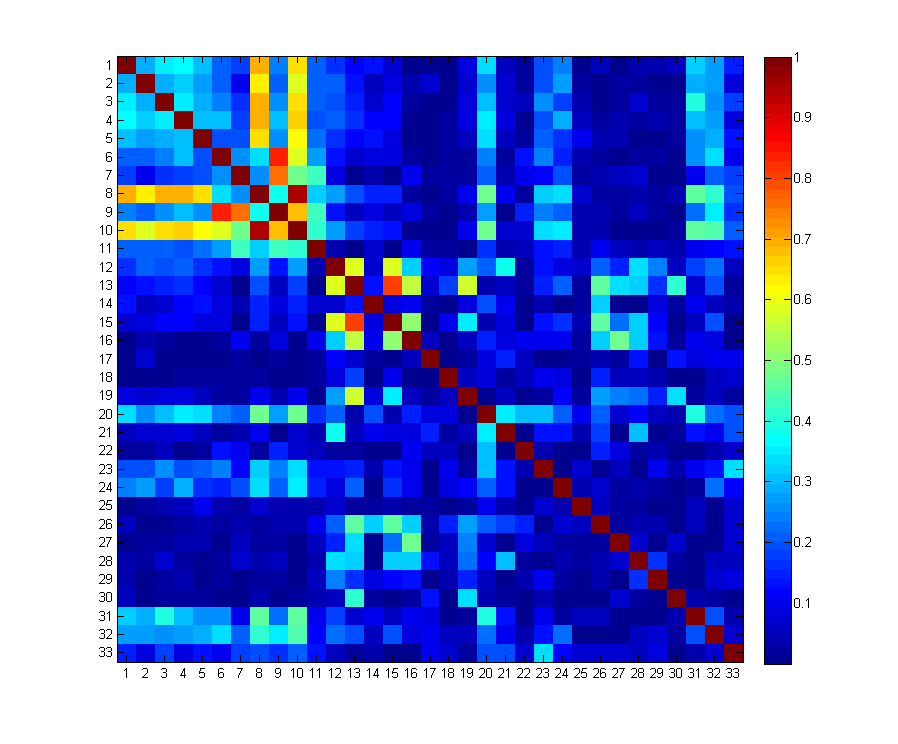
\includegraphics[width = 4cm, height = 3cm]{cov.png}
    \label{fig:cov}
\caption{Example of Covariance Matrix Plot}
(\href{https://www.mathworks.com/matlabcentral/answers/196574-factor-analysis-a-covariance-matrix-is-not-positive-definite}{Referenced})

\end{marginfigure}


A correlation matrix is a matrix showing correlation coefficients between sets of variables. Higher magnitude OF correlation coefficients mean that two different data tips are more linearly related to each other. Still, data tips can be strongly related with smaller magnitude correlation coefficients, just not linearly. 

The correlation matrix is:
\[
\textbf{Correlation Matrix(A)}= 
\frac{1}{\sqrt{N}}
\begin{bmatrix}
    \frac{(x_{1}-\mu_{1})(x_{1}-\mu_{1})}{\sigma_{x_1}\sigma_{x_1}}  & \frac{(x_{1}-\mu_{1})(x_{2}-\mu_{2})}{\sigma_{x_1}\sigma_{x_2}} & \dots & \frac{(x_{1}-\mu_{1})(x_{n}-\mu_{n})}{\sigma_{x_1}\sigma_{x_n}} \\
    \frac{(x_{2}-\mu_{1})(x_{1}-\mu_{1})}{\sigma_{x_2}\sigma_{x_1}}  & \frac{(x_{2}-\mu_{2})(x_{2}-\mu_{2})}{\sigma_{x_2}\sigma_{x_2}} & \dots & \vdots \\
    \vdots & \vdots & \ddots & \vdots \\
    \frac{(x_{n}-\mu_{n})(x_{1}-\mu_{1})}{\sigma_{x_n}\sigma_{x_1}}  & \frac{(x_{n}-\mu_{n})(x_{2}-\mu_{2})}{\sigma_{x_n}\sigma_{x_2}} & \dots & \frac{(x_{n}-\mu_{n})(x_{n}-\mu_{n})}{\sigma_{x_n}\sigma_{x_n}} 
\end{bmatrix}
\]


Where $\sigma_{x_n}$ is the standard deviation.


Then, how should we choose what matrix to use for Principal Component Analysis? Covariance matrix is commonly used when variables are on the same scale. If the variables are on different scale, correlation matrix is used. For example, if the variables have different units of measure, such as pounds and inches. Since you cannot compare pounds and inches directly, you should use correlation matrix. If you want to conduct PCA on the temperature data for different cities, since the units of measure are the same (Either Fahrenheit or Celsius), covariance matrix should be used. In cases where scales are different, covariance matrix can also adjust the scales of the variables. For example, if you want to conduct PCA on population for different states, using covariance matrix would account for the size of each state.

\begin{marginfigure}
    \centering
    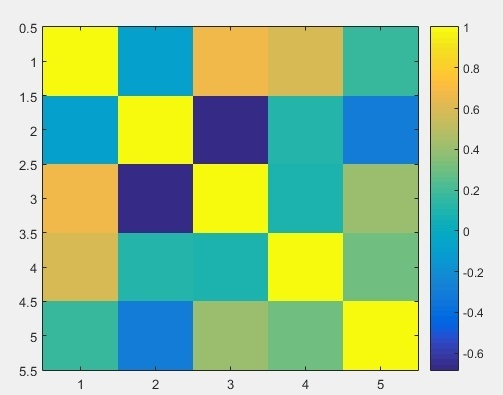
\includegraphics[width = 6cm, height = 5cm]{correlation.jpg}
    \label{fig:corr}
\caption{Example of Correlation Matrix Plot}
(\href{https://www.quora.com/Whats-the-best-way-to-visualize-correlations-between-six-value-vectors}{Referenced})


\end{marginfigure}

\begin{enumerate}
	\item Load sample data in MATLAB by typing \verb|load hospital|. Then, with \verb|[X = hospital.Weight, hospital.BloodPressure]|, plot the correlation and covariance matrix of the data and find how weight and blood pressure are related. Also, state how correlation and covariance matrix are different.
\end{enumerate}

\begin{marginfigure}
    \centering
    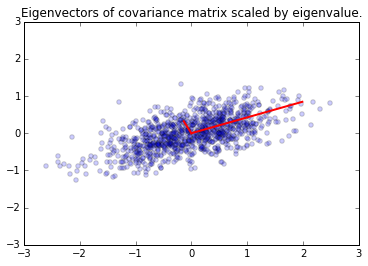
\includegraphics[width = 6cm, height = 5cm]{PCA.png}
    \label{fig:PCA}
\caption{Example of PCA}
(\href{https://people.duke.edu/~ccc14/sta-663/PCASolutions.html}{Referenced})

\end{marginfigure}

\subsection{Principal Component Analysis - Singular Value Decomposition}
Helpful Resource: 
\href{https://www.cs.cmu.edu/~venkatg/teaching/CStheory-infoage/book-chapter-4.pdf}{CMU CS Theory}

Single Value decomposition is decomposition of a matrix M (m by n) whose entries come from the field K, which is either the field of real numbers or the field of complex numbers. The decomposition takes the form of ${\displaystyle \mathbf {M} =\mathbf {U} {\boldsymbol {\Sigma }}\mathbf {V} ^{*}}$, where $\mathbf{U}$ is m by m unitary matrix (if  K = ${\displaystyle \mathbb {R} } \mathbb {R}$ , unitary matrices are orthogonal matrices), $\boldsymbol{{\Sigma}}$ is a diagonal m by n matrix with non-negative real numbers on the diagonal, $\mathbf{V}$ is an n by n unitary matrix over K, and
$\mathbf{{V}^{*}}$ is the conjugate transpose of V.

The diagonal entries ${\sigma_{i}}$ of $\mathbf{\Sigma}$ are known as the singular values of M. A common convention is to list the singular values in descending order. In the other words, the first entry of the singular value (eigenvalue) represents how much of eigenvector corresponding to the eigenvalue is represented in the data. The second entry of the singular value represents the second most eminent direction how data is projected and so on. Therefore, by picking certain number of singular value, you can scale your data set and this process is called Principal Component Analysis. (\href{https://en.wikipedia.org/wiki/Singular-value_decomposition}{Referenced})



\begin{enumerate}
	\setcounter{enumi}{1}
	\item Load sample data in MATLAB by typing \verb|load hald|. Conduct SVD on one of four variables and plot the resultant data. Then, conduct SVD without using SVD command and plot the resultant data. Compare two plots to see if they match. These resources might be helpful: \href{https://www.mathworks.com/help/matlab/ref/svd.html}{SVD MATLAB documentation} and \href{http://www.matrixlab-examples.com/singular-value-decomposition.html}{SVD MATLAB tutorial}

\end{enumerate}


% ----- Audio Preprocessing -----

\section{Frequency Analysis and Filtering (3 hours)}

\subsection{Discrete Fourier Transform (DFT)}
This section reviews and builds off section of the overnight from Module 2 Night 3.

Key ideas reviewed:
\begin{itemize}
	\item You can sample a continuous, real-world signal by sampling at discrete time steps using a simple matrix
	\item You can use these more simple, digital responses to analyze a signal
	\item You can convert a signal in the frequency domain back to the time domain
\end{itemize}

Recall that when a computer (or any digital device) samples an audio source, it samples it at a set frequency, or sampling rate. Basically a computer has a special type of clock in it that allows it to perform sampling operations only a certain number of times during a period of time. 
 
 \begin{marginfigure}
    \centering
    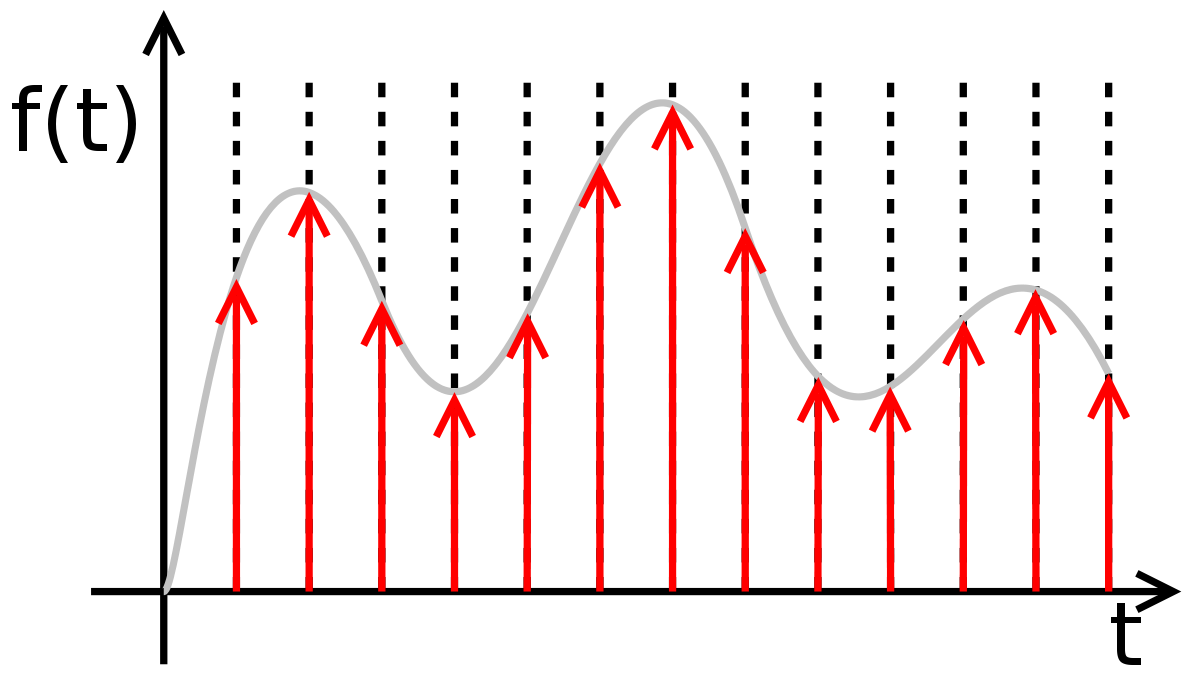
\includegraphics[width = 6cm, height = 4cm]{discrete_time.png}
    \label{fig:discrete_time}
\caption{A continuous signal (in grey) being sampled at a specified sample rate (red arrows).}
	\label{fig:discrete_time}
\end{marginfigure}

As in figure \ref{fig:discrete_time}, a continuous sound signal can be broken up, or sampled, at different points. As you can imagine, if you don't sample at a high enough frequency, you will lose valuable information about your continuous signal. This is called aliasing. As you also might remember, as per the \textit{Nyquist Sampling Theorem}, you only have to sample at twice the frequency of the highest frequency present in your continuous signal to be able to fully reconstruct your continuous signal. 

Once you have turned an analog, continuous signal into a digital, discrete signal in the time domain, you can project it into the frequency domain which allows for rich analysis of the information within the signal. 

If you'd like to watch a quick (4 minute) refresher video on the DFT, \href{https://www.youtube.com/watch?v=h6QJLx22zrE}{here} is a good video that explains how it works.

Recall that the Discrete Fourier Transform (DFT) works by taking a signal and sampling at a certain frequency $Fs$ and then correlating how much of each sinusoidal basis function is in each sample. 

Let's say our sampled signal looks like \ref{eq:sampled_audio} where $N$ is the time where the signal was sampled:
\begin{equation}\label{eq:sampled_audio}
    x=
\begin{bmatrix}
    x[1]       \\
    x[2]       \\
    \vdots \\
    x[N-1]
\end{bmatrix}
\end{equation}

Now we need to generate a matrix of the sinusoidal basis functions which are all just sinusoidal functions that are dependent on how many samples were taken and were they are in the sample range.
\begin{equation}\label{eq:basis_fns}
    W=\dfrac{1}{\sqrt{N}}
\begin{bmatrix}
    1 & 1 & 1 & \dots  & 1 \\
    1 & e^{-\frac{2 \pi j}{N}} & e^{-\frac{2 \pi j}{N}2} & \dots  & e^{-\frac{2 \pi j}{N}(N-1)} \\
    1 & e^{-\frac{3 \pi j}{N}} & e^{-\frac{2 \pi j}{N}2} & \dots  & e^{-\frac{2 \pi j}{N}(N-1)} \\
    \vdots & \vdots & \vdots & \ddots & \vdots \\
    1 & e^{-\frac{(N-1) \pi j}{N}} & e^{-\frac{(N-1) \pi j}{N}2} & \dots  & e^{-\frac{(N-1) \pi j}{N}(N-1)}
\end{bmatrix}
\end{equation}
This vector can then be used to calculate the weights of $W$ on $x$ as
\begin{equation}
a = W x
\end{equation}
Once you get these weights, you can plot them and see the frequency response of the signal in the frequency domain. This is what the \textit{fft()} function does in Matlab.

To covert the signal back to time domain, you can use a similar matrix and the weights to get time function components. 
\begin{equation}\label{eq:basis_fns}
    W^{-1}=\dfrac{1}{\sqrt{N}}
\begin{bmatrix}
    1 & 1 & 1 & \dots  & 1 \\
    1 & e^{\frac{2 \pi j}{N}} & e^{\frac{2 \pi j}{N}2} & \dots  & e^{\frac{2 \pi j}{N}(N-1)} \\
    1 & e^{\frac{3 \pi j}{N}} & e^{\frac{2 \pi j}{N}2} & \dots  & e^{\frac{2 \pi j}{N}(N-1)} \\
    \vdots & \vdots & \vdots & \ddots & \vdots \\
    1 & e^{\frac{(N-1) \pi j}{N}} & e^{\frac{(N-1) \pi j}{N}2} & \dots  & e^{\frac{(N-1) \pi j}{N}(N-1)}
\end{bmatrix}
\end{equation}

\subsection{Noise Removal}
One of the more useful operations in audio processing is the filtering of unwanted noise from an audio sample. In the context of voice recognition, this means removing all extraneous sounds - background noise, microphone hiss, recording artifacts - other than the actual voice that we are trying to isolate. This is particularly relevant to the problem of voice recognition, since we want our program to only match based on the qualities of individual voices, not the conditions of their recordings.

In this section, we will be exploring a few methods of removing unwanted noise using the frequency domain. Using $audioread$ in MATLAB, load the sound sample \verb|NASA_80Hz_2900Hz|. This is a recording of a NASA transmission, but it has been corrupted with two sine wave tones that are playing over the original sample.

\begin{enumerate}
	\setcounter{enumi}{2}
	\item Plot the DFT of the corrupted audio file, and compare it to the clean, original recording (\verb|NASA.wav|). What is different?
	\item How do the frequencies represented in the original audio sample compare to the frequencies added as noise?
\end{enumerate}

One of the simplest filtering techniques is the ideal high-pass and ideal low-pass filters. For an ideal high-pass filter, all frequencies below a certain threshold are completely eliminated from the signal, while frequencies above that threshold are preserved; the opposite is true for an ideal low-pass filter. These can be accomplished either by applying a convolution or by editing the values of the DFT in MATLAB.

\begin{enumerate}
	\setcounter{enumi}{4}
	\item Implement an ideal band-pass filter and apply it to the corrupted NASA transmission. Keep in mind that you don't want to remove the voice from the recording, so you may want to look up what the typical frequency range of a human voice is when determining your threshold frequencies.
	\item Compare the processed recording to the corrupted recording and to the original, uncorrupted recording. What is different? Does your new sample sound different than the clean sample?
	\item What are the limitations of this method of noise filtering?
\end{enumerate}

\subsection{Spectral Subtraction Overview}
As you probably discovered, ideal band-pass filters are very effective at removing background noise from an audio file \textit{provided that it is outside the frequency range of the sounds you want to preserve}. If the noise had been in the frequency range of human speech, it would not have been possible to filter out this way without damaging the original signal.

Spectral subtraction, a different technique which is actually used commonly in audio processing, doesn't have this limitation. It relies on the following assumption:
\begin{equation}
	T[n] = V[n] + N[n]
\end{equation}
Where $T[n]$  is the DFT of the unprocessed sound sample, including unwanted noise, $V[n]$ is the DFT of the voice or other sound sample you want to isolate, and $N[n]$ is some known frequency profile for the background noise you want to remove. If you rearrange this equation, you get the following:
\begin{equation}
	V[n] = T[n] - N[n]
\end{equation}
In other words, to get the voice information on its own, you just need to subtract the unwanted noise from the original sound sample. This is essentially how spectral subtraction works on a high level, and why it can remove background noise indiscriminately of frequency.

There are several useful resources online for spectral subtraction, but \href{http://practicalcryptography.com/miscellaneous/machine-learning/tutorial-spectral-subraction/}{here} is one that I found particularly useful.

\subsection{Spectral Subtraction Implementation}
For this part of the assignment, you will be using spectral subtraction to remove the excess noise from this audio file: \verb|NASA_noisy.wav|. Unlike the previous corrupted recording, this sample has some added radio static that spans the entire frequency domain - including the frequencies represented in the voice itself.

An important step to implementing spectral subtraction is slicing the original sample into several smaller chunks. This helps you better identify and define your noise profile and allows you to operate on samples of arbitrary length.

When determining the length of these slices, there are a few things to keep in mind. Each slice needs to contain a enough information to fully represent your background noise, but at the same time you want shorter samples so that you can fit more in a given time period. I used 0.1 seconds, and it seemed to be a good balance of the two.

Additionally, these samples should not be taken exactly end-to-end, but rather overlap somewhat in their position along the original audio track. For instance, if each sample is 0.1 seconds long, you might have samples every 0.05 seconds which overlap by half. This creates smoother transitions between samples and ensures that you don't lose any important data because it happened to lie on the border between two slices of your sample.

\begin{marginfigure}
    \centering
    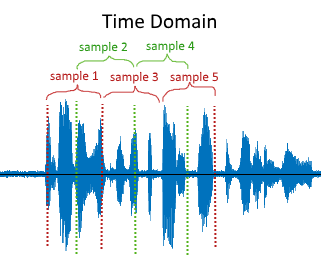
\includegraphics[width = 6cm, height = 5cm]{sample_1.png}
    \label{fig:sample_data_1}
\caption{An example of how you might sample your data.}
\end{marginfigure}

After you slice your sample, you want to find the magnitude and phase of the DFT for the sample, as well as for a section of the sample that contains only noise (in the case of the noisy NASA transmission, the first approximately 4.5 seconds are noise, while the last 4.5 seconds are speech). You ultimately want to end up with the following three matrices:

\begin{equation}\label{eq:sampled_audio}
    T_M=
\begin{bmatrix}
    T_{MS1}       \\
    T_{MS2}       \\
    \vdots \\
\end{bmatrix}
	T_\theta=
\begin{bmatrix}
    T_{\theta S1}       \\
    T_{\theta S2}       \\
    \vdots \\
\end{bmatrix}
	N_M=
\begin{bmatrix}
    N_{MS1}       \\
    N_{MS2}       \\
    \vdots \\
\end{bmatrix}
\end{equation}

Where $T_M$ is a matrix of all the magnitudes of the DFTs of each slice in your sample, $T_\theta$ is a matrix of all the phase information of the DFTs of each slice in your sample, and and $N_M$ is a magnitude matrix similar to $T_M$ but sampled from a part of the recording that contains only noise. The MATLAB functions abs and angle will be useful for determining magnitude and phase, respectively, of a matrix of complex numbers.

Next, we want to determine the average frequency profile of the background noise in our audio file. This will functionally act as the N[n] term that you saw in the first equation, and we will later subtract it from our other data matrix. In this case, we can just find an average:
\begin{equation}
	N_{MA} = \frac{1}{n}\sum_{}^{} N_{MR}
\end{equation}

Where $n$ is the number of slices in your sample of background noise and $N_{MR}$ is the element of $N_M$ in row R. We can then subtract this ``average noise`` from each sample of our full sample magnitude matrix, with a weight:
\begin{equation}
	T_{M_{clean}} = (1-h)T_M - h*N_{MA} = 
	\begin{bmatrix}
    (1-h)T_{MS1} - h*N_{MA}       \\
    (1-h)T_{MS2} - h*N_{MA}       \\
    \vdots \\
\end{bmatrix}
\end{equation}

Where $h$ is a semi-arbitrary ``noise-to-sound ratio`` The higher this value, the more noise you remove, and the more you damage the original signal. I used a value of 0.7, but it is worth experimenting with this to see how it affects your results.

You also want to make sure that your filtered matrix is always at least zero, because it is the magnitude of your complex DFT values (and a negative magnitude doesn't make sense in this context). You can treat it like a piece wise function: \\
\begin{figure}
	\centering 
	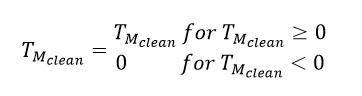
\includegraphics[width=0.7\textwidth]{piecewise.png}
	\label{fig:piecewise}
 \end{figure}
This gives us the magnitudes of the slice DFTs for a filtered recording. We can use these magnitudes, and the phases we recorded earlier, to obtain the complex values of the DFT:
\begin{equation}
	T_{clean} = T_{M_{clean}}e^{jT_\theta}
\end{equation}
From there, you just need to compute the inverse DFT of each sample and combine the time-domain samples in a useful way.
\begin{enumerate}
	\setcounter{enumi}{7}
	\item Plot the filtered and unfiltered sound in time and frequency domain. How did the spectral subtraction affect the signal?
	\item Listen to your filtered sound and to \verb|NASA.wav| How are they different? Try adjusting your parameter for slice length and see how that affects this difference.
	\item Apply this technique to \verb|NASA_80Hz_2900Hz|. How does it compare to the ideal band-pass filter for filtering out the two sinewaves?
	\item Try one of the modifications to spectral subtraction described in the ``Modifications`` section of the \href{http://practicalcryptography.com/miscellaneous/machine-learning/tutorial-spectral-subraction/}{linked page}. How does this effect the quality of noise removal?
\end{enumerate}

% ----- Audio Preprocessing -----

\section{Audio Preprocessing (2 hours)}

As you learned in the previous section, audio clips can be quite unclean when they are recorded. Let's say, for example, that we want to build a database of short clips of people saying a single word. This database might be used to train and test an algorithm such as the one we developed before. In our case, here's what we have:
\begin{itemize}
	\item 30 People
	\item 8 words
	\item Each word repeated 3 times
	\item Each clip lasts 3 seconds
\end{itemize}
This gives us quite a nice set of data, but it's very messy. The provided audio samples were recorded in a pretty loud hallway where people can be heard talking, doors closing, and people walking. In addition, you might notice that each person doesn't say their word at exactly the same time as everyone else. As you can see in figure \ref{fig:time_graphs}, the part of the clip where the person speaks (as characterized by the jump in levels) starts at slightly different times.
\begin{marginfigure}
	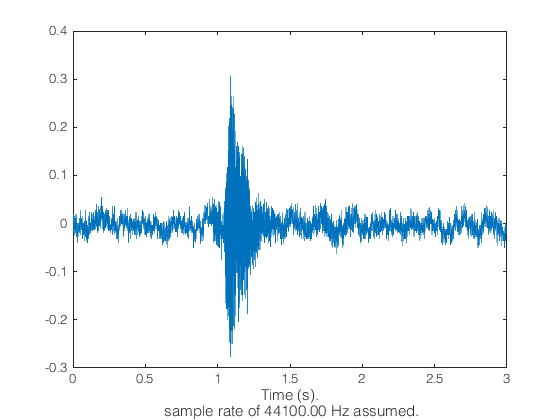
\includegraphics[width = 6cm, height = 5cm]{time_1.png}
	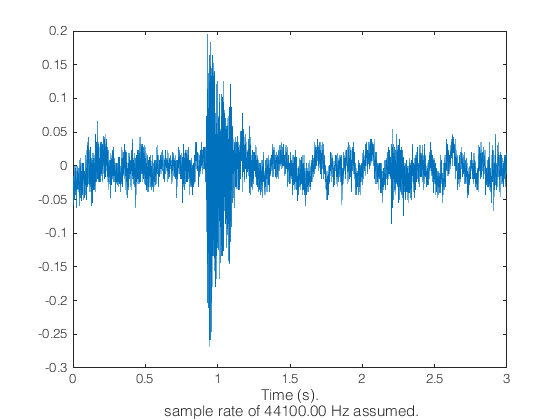
\includegraphics[width = 6cm, height = 5cm]{time_2.png}
	\caption{Two raw audio clips before processing}
	\label{fig:time_graphs}
\end{marginfigure}

\subsection{Algorithm Creation}
To start trimming these clips to length, we should start by observing them. Obviously the levels of the word are significantly higher than other times during the clip. However, some clips have more fluctuation in their levels surrounding the words, so we'll need to apply our filtering.


\begin{marginfigure}
	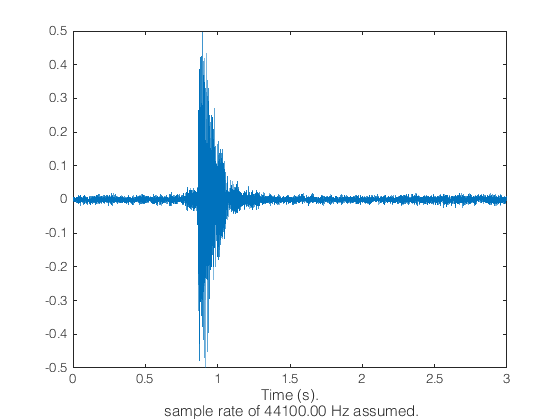
\includegraphics[width = 6cm, height = 5cm]{cleaned_time_2.png}
	\caption{Audio clip after being filtered with a band-pass filter}
	\label{fig:cleaned_time_graphs}
\end{marginfigure}
After filtering is done (as can be seen in figure \ref{fig:cleaned_time_graphs}), after applying the band pass filter, our data is significantly cleaner and devoid of noise. This helps our 'word part' stand out much more.

To isolate the word consistently, we shall define a threshold and gather a section of the clip surrounding the point where this threshold is triggered. In essence, we will look through all the sample points of the signal and when the level goes above 0.1, we shall take out a sub clip of 0.5s surrounding that point. 

\begin{enumerate}
	\setcounter{enumi}{11}
	\item Build an algorithm to trim all the sound clips to be the same length and contain the word part. Work on this for an hour, and if you do not come up with something, feel free to use the sample script found \href{#}{here}. We don't want you to struggle on a relatively simple algorithm, but feel it would help familiarize you with the format of the data sets. 
\end{enumerate}


\subsection{Finding Average Voice \& Going Further}
% Finding Average Face
\begin{enumerate}
	\setcounter{enumi}{12}
	\item Just as you did in the \textit{Eigen Analysis Revisited} section, we're going to find the average voice of the data set. Here's an overview of what we'd like you to do: \\ 
	\begin{itemize}
		\item Filter the audio and trim it to length
		\item Add all clips together (in the frequency domain, of course!) and divide by the number of clips. 
		\item Take an inverse fourier transform of this new clip and listen to it.
		\item Describe what you hear and think about why it sounds the way it does.
	\end{itemize}
\end{enumerate}

% Go further
\begin{enumerate}
	\setcounter{enumi}{13}
	\item \textit{Optional:} Now that you have found the average voice, feel free to try the eigen analysis section using the sound data sets and the average voice you just found. 
\end{enumerate}

\end{document}



